
\begin{figure}
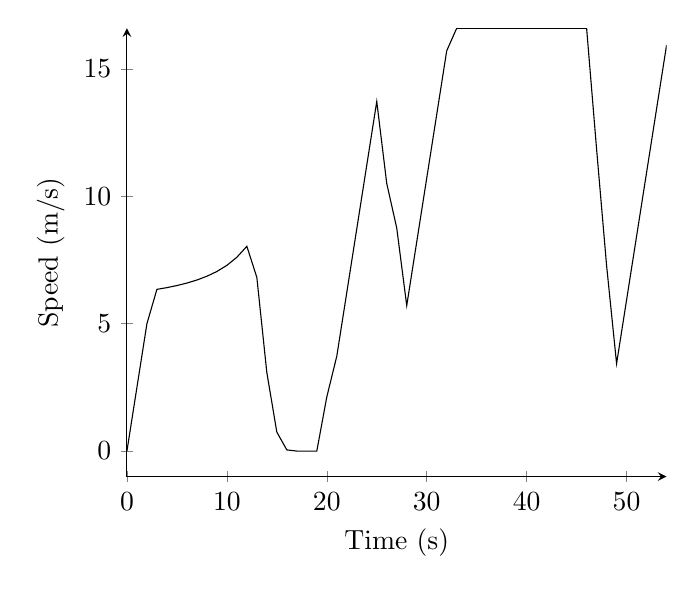
\begin{tikzpicture}
\begin{axis}[
legend style={anchor=west},
axis x line=bottom,
axis y line=left,
ymin=-1,
xlabel=Time (s),
ylabel=Speed (m/s),
]
\addplot[] coordinates {
(0, 0.0)
(1, 2.5)
(2, 5.0)
(3, 6.34875857266)
(4, 6.41666409566)
(5, 6.49767405968)
(6, 6.59541081725)
(7, 6.71484941477)
(8, 6.86297709817)
(9, 7.04986402536)
(10, 7.29046911431)
(11, 7.60782545253)
(12, 8.03896822491)
(13, 6.81883328269)
(14, 3.0827576945)
(15, 0.745620431289)
(16, 0.0461516543629)
(17, 0.0)
(18, 0.0)
(19, 0.0)
(20, 2.12416949449)
(21, 3.72358364023)
(22, 6.22358364023)
(23, 8.72358364023)
(24, 11.2235836402)
(25, 13.7235836402)
(26, 10.5047984324)
(27, 8.75533134267)
(28, 5.7120238684)
(29, 8.2120238684)
(30, 10.7120238684)
(31, 13.2120238684)
(32, 15.7120238684)
(33, 16.6)
(34, 16.6)
(35, 16.6)
(36, 16.6)
(37, 16.6)
(38, 16.6)
(39, 16.6)
(40, 16.6)
(41, 16.6)
(42, 16.6)
(43, 16.6)
(44, 16.6)
(45, 16.6)
(46, 16.6)
(47, 11.8462901184)
(48, 7.27910349267)
(49, 3.43320452747)
(50, 5.93320452747)
(51, 8.43320452747)
(52, 10.9332045275)
(53, 13.4332045275)
(54, 15.9332045275)
};

\end{axis}
\end{tikzpicture}
\label{tik:speed:100:68}
\caption{100 percent diving with GSC on route $68$}
\end{figure}
